\documentclass[a4paper]{book}
\usepackage{graphicx}
\usepackage{caption}
\usepackage{subcaption}
\usepackage{amsmath}
\usepackage{letltxmacro}
\usepackage{mathtools}
\usepackage{braket}
\usepackage{svg}
\usepackage{hyperref}
\usepackage[style=numeric, sorting=none]{biblatex}
\addbibresource{master_thesis.bib}
\everymath{\displaystyle} % make math symbols in line slightly bigger in the all text

\newcommand{\sss}{\;\;\;} % spacespacespace for conditions in equations e.g. for E << kT
\newcommand{\tsub}{\textsubscript}
\newcommand{\mb}{\mathbf}
\newcommand{\mbe}{\mathbf{e}}

\usepackage{caption}
\captionsetup{font=footnotesize} % font of figure caption set to footnotesize

\usepackage{fancyhdr}
\setlength{\headheight}{15pt}
\pagestyle{fancy}
\renewcommand{\chaptermark}[1]{ \markboth{#1}{} }
\renewcommand{\sectionmark}[1]{ \markright{#1} }
\fancyhf{}
\fancyfoot[LE,RO]{\thepage}
\fancyhead[LE]{\ifnum\value{chapter}>0 \MakeUppercase{\chaptername} \thechapter. \fi  \textit{ \nouppercase{\leftmark}} }
\fancyhead[RO]{\arabic{chapter}.\arabic{section}. \textit{ \nouppercase{\rightmark}} }
\fancypagestyle{plain}{ %
	\fancyhf{} % remove everything
	\fancyfoot[LE,RO]{\thepage}
	\renewcommand{\headrulewidth}{0pt} % remove lines as well
	\renewcommand{\footrulewidth}{0pt}
}

\begin{document}
	\begin{titlepage}
		\thispagestyle{empty}
		\centering
		
\includegraphics[width=\textwidth]{images/fu_logo}\par\vspace{1cm}
		{\scshape\LARGE Freie Universität Berlin \par}
		\vspace{1cm}
		{\scshape\Large Master thesis \par}
		\vspace{1.5cm}
		{\huge\bfseries Electrical detection of spins in solar cells \par}
		\vspace{2cm}
		{\Large\itshape Gianluca Marcozzi \par}
		%		\vfill
		%		supervised by\par
		%		Dr.~Mark \textsc{Brown}
		\vfill
		% Bottom of the page
		{\large \today\par}
	\end{titlepage}
	
	\thispagestyle{empty}
	\null\vfill
	\begin{center}
		{\large First supervisor: Prof. Dr. K. Lips\\
			Second supervisor: Prof. Dr. T. Kampfrath \par}
	\end{center}
	\clearpage
	
	\setcounter{page}{1}
	
	\clearpage
	\tableofcontents
	
	% Somewhere here: costants??
	
	\chapter{Introduction}
	Solar energy plays a central role in the perspective of shifting to carbon neutral energy production. In the period between 2008 and 2018, the electricity generated in the EU from solar photovoltaics increased by 15.5 times, reaching around $10^3 \; \text{TWh}$ of energy produced in 2018 \cite{ahmadRecentAdvancesApplications2020}. Nevertheless, this is still less than 4\% of the 2018 gross yearly electricity production in the EU \cite{statisticalofficeoftheeuropeanunionEnergyBalanceSheets2020}.\\
	%	 The current record solar electrical conversion efficiency for c-Si solar cell is 26\% \cite{haaseLaserContactOpenings2018}, while multijunction solar cells with III-V layers achieved 47\% conversion efficiency under light concentration and 39\% under 1-Sun.\\
	In order to make photovoltaics more competitive in the energy market, reduction of material cost and improvement of the photovoltaic efficiency are at the center of the research focus. In this perspective, deeper physical understanding of the processes involved in charge transport in solar cells will provide the basis for improvement of existing technologies \cite{schneggPulsedElectricallyDetected2012}\cite{behrendsSpindependentTransportRecombination2009}.\par
	
	In the world, around 95\% of the solar cells are based on crystalline silicon (c-Si) wafer technology \cite{InternationalTechnologyRoadmap2021}. Record efficiency for c-Si solar cells reaches values of 26.7\% in the laboratory and 24.4\% for module sizes \cite{greenSolarCellEfficiency2021}, approaching the theoretical limit of 29\% for single-junction c-Si solar cells due to Schockley-Queisser limit and Auger recombination \cite{richterReassessmentLimitingEfficiency2013}. Nevertheless, a complete understanding of the microscopic nature of the physical processes that limit the efficiency of the solar cell is missing.\par
	
	The main part of this work is therefore dedicated to the study of electronic transitions in solar cells with c-Si absorbers. In particular, the spin-dependent nature of the interaction between charge carriers and localized defects will be investigated. These defects act as recombination centers for free charge carriers, reducing the photoconductivity, hence the efficiency, of the solar cell \cite{moserChargeTransportAmorphous2019}. Due to their paramagnetic nature, these defects can be studied through the well established experimental technique of electron paramagnetic resonance (EPR) \cite{meyerAtomicStructureLightinduced2021}\cite{lenahanWhatCanElectron1998}. Nevertheless, the spectroscopic technique of choice in the frame of this work is electrically detected magnetic resonance (EDMR) because it directly probes the current-limiting charge-transport processes through paramagnetic defects. EDMR provides also high sensitivity (up to single spin detection \cite{xiaoElectricalDetectionSpin2004}), enabling the measurement of state of the art solar cells with low density of defects \cite{schneggPulsedElectricallyDetected2012}. \par
	
	Additionally, a small part of this project will focus on the production of a heterojunction intrinsic layer (HIT) solar cell. In these devices, layers of intrinsic amorphous silicon (a-Si) are evaporated on both sides of a c-Si absorber. Highly doped hydrogenated amorphous silicon (a-Si:H) layers are used as selective contacts. This structure has been shown to improve the efficiency of c-Si based solar cells \cite{taguchiHITTMCellsHighefficiency2000}.
	Previous research shows that defects at the interface between c-Si and a-Si induced by the structural discontinuity can act as recombination centers, limiting the efficiency of the solar cell \cite{georgeAtomicStructureInterface2013}.
	Moreover, conductive atomic force microscopy (AFM) measurements allowed to identify electronic transitions through energy levels of the a-Si layers which lower the selectivity of the contacts, therefore leading to a decrease of the efficiency of the device \cite{teferiImagingBandtailStates2021}. In the perspective of deepening the knowledge about this processes through EDMR measurements, the production of such HIT solar cells will be carried out in the frame of this project. After the realization of these samples, EDMR measurements should allow to characterize the recombination processes that take place in the a-Si layers.
	%Thin-film solar cells offer good potential as a low-cost technology. Taking advantage of the optical properties of  
	\\
	
	\chapter{EPR and EDMR}
	% Riassunto di quello che dico nel capitolo?
	The first part of this work focuses on the study of spin-dependent charge-transport through paramagnetic defects in state of the art solar cells. The experimental technique of choice is electrically detected magnetic resonance (EDMR) because it provides the selectivity and sensitivity required to carry out this investigation \cite{schneggPulsedElectricallyDetected2012}.
	%Nevertheless, it is necessary to have a good understanding of Electron Paramagnetic Resonance (EPR), which is the spectroscopic technique on which EDMR is based, is necessary to be able to interpret correctly any EDMR spectrum.
	Since EDMR is based on electron paramagnetic resonance (EPR), a good understanding of the latter is necessary to be able to correctly interpret EDMR spectra. The following chapter is therefore dedicated to the description of the fundamental principles of EPR and EDMR.\\\\
	
	
	\section{Basic principles of EPR}
	\label{sec:2_basic_principles_EPR}
	The electron carries an intrinsic angular momentum, the quantum spin $\mb{S}$. The magnetic moment of the electron is given by the expression:
	\begin{equation}
		\boldsymbol\mu = \gamma\hbar\mb{S} = g\frac{-e\hbar}{2m\tsub{e}}\mb{S} = -g\mu\tsub{B}\mb{S},
		\label{eq:2_electron_mu}
	\end{equation}
	where $\gamma = g\mu_B/\hbar$ is the gyromagnetic ratio, $\mu_B = e\hbar/2m_e $ is the Bohr magneton, $\hbar=h/2\pi$ is the reduced Planck constant, $m_e$ is the mass of the electron and $g$ is the electron $g$-value. For a free electron, the g-value is equal to $g_e \simeq 2.002319$. If the electron is bound to a nucleus or is subject to local fields generated by a crystal lattice, then its g-value deviates from the value of the free electron value.
	
	When an external magnetic field $\mb{B}_0 = B_0\mbe_z$ is present, the spin aligns either parallel or antiparallel to the direction of the field. The two configurations are associated with two different energy states, as described by the Zeeman Hamiltonian:
	\begin{equation}
		\mathcal{H}\tsub{Z} =
		-\boldsymbol\mu\cdot\mb{B}_0 =
		g\mu\tsub{B}\mb{S}\cdot\mb{B}_0 =
		g\mu\tsub{B}S_{z}B_0 =
		m\tsub{S}g\mu\tsub{B}B_0,
		\label{eq:2_Hz_free}
	\end{equation}
	where $m_S = +1/2$ for spin parallel to the magnetic field and $m_S = -1/2$ for antiparallel. For $B_0 = 0$, the two spin states are degenerate. For $B_0 \neq 0$, the interaction with the magnetic field lifts the spin degeneracy, giving rise to an energy splitting between the states equal to:
	\begin{equation}
		\label{eq:2_Zeeman_splitting}
		\Delta E = g\mu\tsub{B}B_0.
	\end{equation}
	Due to this energy difference, the occupation of two Zeeman levels will be different. At thermal equilibrium, the number of electrons with spin up $N_\uparrow$ and with spin down $N_\downarrow$ are described by Boltzmann statistics:
	\begin{equation}
		\frac{N_\uparrow}{N_\downarrow} =
		\exp\left(-\frac{\Delta E}{kT}\right),
	\end{equation}
	where $k$ is the Boltzmann constant and $T$ is the temperature.
	
	In an EPR experiment, transitions between the two Zeeman states are induced using electromagnetic radiation of energy $h\nu$. Due to the difference of occupation between the two states, irradiation of the sample with microwave radiation of appropriate frequency will lead to absorption. In particular, the transition between the two energy levels is achieved when the frequency of the external microwave radiation is equal to:
	\begin{equation}
		\label{eq:2_nu_equal_nuL}
		\nu = \nu \tsub L = \Delta E/h = g\mu\tsub B B_0 / h,
	\end{equation}
	where $\nu\tsub L$ is the so-called Larmor frequency.\\
	During a cwEPR experiment, the microwave frequency $\nu$ is kept constant while the external magnetic field $\mb{B}_0$ is swept adiabatically, thus changing the value of the Larmor frequency $\nu\tsub L$, so that an absorption peak can be observed when the conditions in Eq. \eqref{eq:2_nu_equal_nuL} are met. The most commonly used microwave sources are X-Band sources, that is they have frequency $\nu \simeq 9.6 \; \text{GHz}$, which leads to a resonant magnetic field $B_0 \simeq 340 \; \text{mT}$ for the free electron.
	
	Transitions between states take place only when a population difference is established between the two energy levels. An important quantity to take into consideration is thus the spin polarization:
	\begin{equation}
		\frac{\Delta N}{N\tsub{S}} =
		\frac{N_\downarrow - N_\uparrow}{N_\downarrow + N_\uparrow} =
		\frac{1 - \exp(- \Delta E/kT)}{1 + \exp(- \Delta E/kT)} \simeq
		\frac{\Delta E}{2 kT} \sss \text{(for $\Delta E \ll kT$)},
		\label{eq:2_spin_polarization}
	\end{equation}
	where $N_S$ is the total number of spins in both energy levels. At room temperature, the value of the thermal energy is $kT \simeq 25 \; \text{meV}$, while for X-Band the energy difference between the two Zeeman levels is $\Delta E = g\mu_BB_0 \simeq 4 \cdot 10^{-2} \; \text{meV}$, thus fulfilling the condition in brackets in Eq. \eqref{eq:2_spin_polarization}. In this case, the spin polarization is $\Delta N/N_S \simeq 8\cdot10^{-4}$. At a temperature $T = 5 \; \text{K}$ the thermal energy will be equal to $kT \simeq 0.4 \; \text{meV}$, which leads to a larger spin polarization $\Delta N/N_S \simeq 5\cdot10^{-2}$.\\
	Thus, the intensity of the EPR signal is proportional to the population difference \cite{athertonPrinciplesElectronSpin1993}:
	\begin{equation}
		I \propto \Delta N \simeq
		\frac{\Delta E}{2kT}N\tsub{S} \sss \text{(for $\Delta E \ll kT$)}.
		\label{eq:2_I_propto_dN}
	\end{equation}
	The use of a cryostat to reach low temperature leads to an increase of signal of almost two orders of magnitude. Moreover, as shown in Eq. \eqref{eq:2_I_propto_dN}, the intensity of the signal is proportional to the total number of spins in the sample $N_S$. This means that EPR can be used to gain information about the total amount of paramagnetic centers.
	
	\section{Spin dynamics in magnetic fields}
	Most EPR experiments reported are cwEPR, in which microwave irradiation at a fixed frequency is used and the magnetic field is swept adiabatically. Nevertheless, to study the dynamics and the coherence of the spin system it is useful to conduct pulsed EPR (pEPR) experiments \cite{stollPulseEPR2017}. In these experiments, a sequence of short ($\sim \text{ns}$) high-intensity microwave pulses are used to bring the system to a non-equilibrium state. pEPR allows the resolution of small interactions which are unresolved in cwEPR spectra and the disentanglement of overlapping signals. Moreover, properties like relaxation times of the spin species can be obtained by recording the transient response back to the equilibrium state ($\sim\mu\text{s}$) \cite{stollPulseEPR2017}.\\
	
	\subsection{Classical description of EPR}
	\label{sec:2_classical_description}
	In order to study the dynamics of spins in an external magnetic field, it is helpful to approach the process from a classical description. 
	%This is the path that in 1946 lead Felix Bloch to the development of the so-called Bloch equations.
	\\
	Firstly, let us consider the total magnetic moment $\mb M$ of a system of $N_S$ spins $S = 1/2$. In the presence of an external magnetic field $\textbf{B}_0 = B_0\mbe_z$, using Eq. \eqref{eq:2_spin_polarization} one can obtain the value of magnetic moment at thermal equilibrium $\mb M_0$, which is given by the Curie law:
	\begin{equation}
		\label{eq:2_Curie_law}
		\mb{M}_0 = 
		\sum^{N_S}_{i = 1} \boldsymbol \mu_i =
		M_0\textbf{e}_z \simeq		
		-N\tsub S\frac{g^2\mu^2\tsub B B_0}{4kT}\mbe_z.
	\end{equation}
	Considering the more general case of a time dependent magnetic field $\mb{B}(t)$, the equation of motion for the magnetic moment is given by:
	\begin{equation}
		\label{eq:2_eq_motion_M}
		\frac{d\mb{M}}{dt} = 
		\gamma\mb{B}(t)\times\mb{M},
	\end{equation}
	which describes the precession of $\mb{M}$ about the magnetic field axis. Of particular interest is the case in which the magnetic field is the sum of two terms:
	\begin{equation}
		\mb{B}(t) = \mb{B}_0 + \mb{B}_1(t) = B_0 \textbf{e}_z + B_1[\cos(\omega t)\mbe_x + \sin(\omega t)\mbe_y],
		\label{eq:2_B_B0_B1t}
	\end{equation}
	where $\mb B_0$ is a constant field along the $z$-axis, while $\mb B_1(t)$ is a circularly polarized magnetic field rotating counter-clockwise in the $xy$-plane with a frequency $\omega = 2\pi\nu$. When dealing with EPR, $\mb B_0$ commonly refers to the static field created by the magnet which lifts the spin-degeneracy and establishes the Zeeman splitting, while $\textbf{B}_1(t)$ to the field generated by the microwave radiation.\\
	\begin{figure}
		\centering
		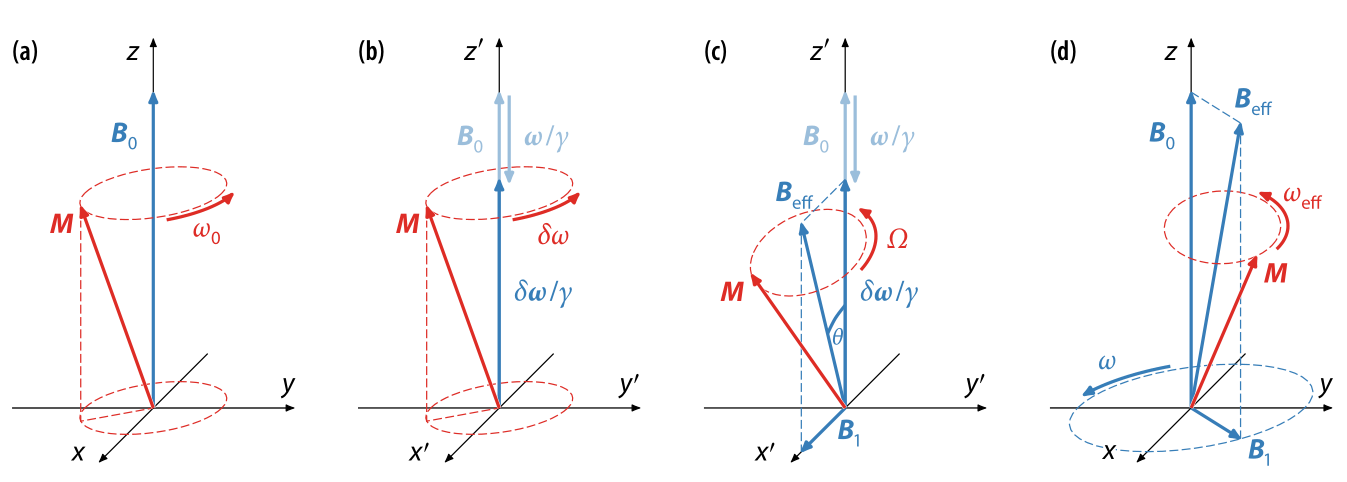
\includegraphics[width=\textwidth]{images/2_rotating_frame}
		\caption{Illustration of the dynamics of the magnetic moment vector in the laboratory and in the rotating frame. (a) If an external magnetic field $\mb B_0 = B_0\mbe_z$ is present, in the laboratory frame the magnetic moment $\mb M$ precesses about the $z$-axis with the Larmor frequency $\omega_0 = 2\pi\nu_0 = \gamma B_0$. (b) In a frame rotating with a frequency $\omega = 2\pi\nu$ around the $z$-axis, the precession frequency is equal to the offset $\delta\omega = \omega_0 - \omega$. (c) If a circularly polarized magnetic field $\mb B_1(t)$ has frequency $\omega$ in the laboratory frame, it will be time independent in the rotating frame. The magnetic moment precesses about the effective magnetic field $\mb B\tsub{eff}$, which forms an angle $\theta$ with the $z$-axis, at the Rabi frequency $\Omega$. (d) In the laboratory frame, the motion of the magnetic moment is a precession about $\mb B\tsub{eff}$ at a frequency $\omega\tsub{eff} = (\nu_0^2 + \nu_1^2)^{1/2}$, superimposed by the precession of $\mb B\tsub{eff}$ about the $z$-axis at a frequency $\omega$. Taken from \cite{moserChargeTransportAmorphous2019}}
		\label{fig:2_rotating_frame}
	\end{figure}
	Due to the rotation of $\mb B_1$, the trajectory of the magnetic moment is a nutation in three dimension. To have a better picture, it is helpful to change the frame of reference to a coordinate system rotating about the $z$-axis with frequency $\omega$.\\
	The axes of the new coordinate system are defined as:
	\begin{subequations}
		\label{eq:2_rotating_frame}
		\begin{align}
			\mbe_x' & = \cos(\omega t)\mbe_x + \sin(\omega t)\mbe_y,\\
			\mbe_y' & = - \sin(\omega t)\mbe_x + \cos(\omega t)\mbe_y,\\
			\mbe_z' & = \mbe_z,
		\end{align}
	\end{subequations}
	which leads to a constant magnetic field:
	\begin{equation}
		\label{eq:2_B_rotating_frame}
		\mb B' = B_0 \mbe_z' + B_1 \mbe_x'.
	\end{equation}
	In the rotating frame, a term needs to be added to the equation of motion to account for the non-inertiality of the frame\footnote{From now on, in this chapter we will refer to the quantities in the rotating frame without explicitly labeling them with a prime $'$.}:
	\begin{equation}
		\frac{d\mb{M}}{dt} = \gamma\mb{B}\times\mb{M} - \boldsymbol \omega \times \mb{M} = (\boldsymbol \omega_0 - \boldsymbol \omega + \boldsymbol \omega_1) \times \mb M,
		\label{eq:2_eq_motion_M_rot}
	\end{equation}
	where $\boldsymbol \omega = \omega \mbe_z$ is the frequency vector that defines the rotation of the new coordinate system, while $\boldsymbol \omega_0 = 2\pi\nu_0 \mbe_z = \gamma B_0 \mbe_z$ and $\boldsymbol \omega_1 = 2\pi\nu_1 \mbe_x = \gamma B_1 \mbe_x$ are the Larmor frequencies of $\mb{B}_0$ and $\mb{B}_1$ respectively.\\
	Eq. \eqref{eq:2_eq_motion_M_rot} describes the so-called Rabi nutation around an effective field:
	\begin{equation}
		\mb{B}\tsub{eff} = \mb{B}_0 - \frac{\boldsymbol \omega}{\gamma} + \mb{B}_1,
		\label{eq:2_Beff}
	\end{equation}
	which forms an angle with the $z$-axis:
	\begin{equation}
		\theta = \arctan\left(\frac{\nu_1}{\delta \nu}\right),
		\label{eq:2_Beff_angle}
	\end{equation}
	where $\delta\nu = \nu_0 - \nu$ is the difference between the Larmor frequencies of $\mb{B}_0$ and the microwave field.\\
	The Rabi frequency, that is the rotation frequency of $\mb{M}$ about $\mb{B}\tsub{eff}$, is the module of the sum of the frequency vectors:
	\begin{equation}
		\Omega = \sqrt{\nu_1^2 + \delta\nu^2}.
		\label{eq_2_rabi_frequency}
	\end{equation}
	In case of resonant microwave ($\delta\nu = 0$), the magnetic moment simply makes a precession about $\mb B_1$ with a frequency $\Omega = \nu_1$. A sketch of the dynamics of the magnetization vector is shown in Fig. \ref{fig:2_rotating_frame}.\\
	The derivation that was proposed until here does not take into account the loss of coherence of the spin system and the relaxation of the magnetic moment towards equilibrium. These phenomena do not have a direct classical interpretation, therefore phenomenological relaxation terms must be considered. Along the $z$-axis, the magnetic moment can be expected to relax exponentially towards the equilibrium value $M_0$ with a spin-lattice, or longitudinal time constant $T_1$. This process can be explained in a quantum mechanical picture as spin-flips from the state with higher energy (spin parallel to the $z$-axis) to the one with lower energy (spin antiparallel to the $z$-axis) through the emission of phonons.\\
	In the $xy$-plane, one can assume exponential decay with a spin-spin, or transverse relaxation time constant $T_2$. The loss of coherence in the transverse plane is due to a modulation of the Zeeman splitting from local field inhomogeneities generated by other spins, which lead to a distribution of individual precession rates. This process does not involve transitions of spins between levels, therefore $T_2$ can be considered different from $T_1$.\\
	Adding these relaxation terms to Eq. \eqref{eq:2_eq_motion_M_rot} leads to the rotating-frame Bloch equations:
	\begin{subequations}
		\label{eq:2_Bloch_eq}
		\begin{align}
			%		\label{eq:2_Bloch_eq_x}
			\frac{dM_{x}}{dt} & = - \delta \omega M_{y} - \frac{M_{x}}{T_2},\\
			%		\label{eq:2_Bloch_eq_y}
			\frac{dM_{y}}{dt} & = \delta \omega M_{x} + \omega_1 M_{z} - \frac{M_{y}}{T_2},\\
			%		\label{eq:2_Bloch_eq_z}
			\frac{dM_{z}}{dt} & = \omega_1 M_{y} - \frac{M_{x}}{T_1}.
		\end{align}
	\end{subequations}	
	%	where $T_1$ is the spin-lattice, or longitudinal relaxation time, and $T_2$ is the spin-spin, or transverse relaxation time. In a quantum mechanical picture, the first one would correspond to spin-flips from the state with higher energy (spin parallel to the $z$-axis) to the one with lower energy (spin antiparallel to the $z$-axis). This can happen due to interaction of the spin with the lattice through emission of phonons. Hence, the component along the $z$ axis is supposed to decay exponentially toward the equilibrium value $M_0$. The second term, $T_2$, is the spin-spin relaxation time. It takes into account the loss of coherence in the $xy$-plane due to local interactions between the spins, which modify their individual precession rates. In a quantum mechanical picture, this would correspond to a modulation of the Zeeman splitting, and doesn't involve transitions of spins between levels. \textbf{citation of Atherton?}.
	The Bloch equations completely describe the spin dynamics of a two-level system. Their solutions are supepositions of nutation and exponential relaxation of the magnetic moment vector components.
	
	\subsection{Continuous wave EPR}
	\label{sec:2_cwEPR}
	In a  continuous wave EPR (cwEPR) experiment, the magnetic moment is given by the steady-state solution of the Bloch equations \eqref{eq:2_Bloch_eq}:
	\begin{subequations}
		\label{eq:2_Bloch_eq_sol}
		\begin{align}
			%		\label{eq:2_Bloch_eq_x_sol}
			M_{x} & = \frac{\delta \omega \, \omega_1T_2^2}{1 + \delta\omega^2 T_2^2 + \omega_1^2T_1T_2}M_0,\\
			%		\label{eq:2_Bloch_eq_y_sol}
			M_{y} & = \frac{\omega_1T_2}{1 + \delta\omega^2 T_2^2 + \omega_1^2T_1T_2}M_0,\\
			%		\label{eq:2_Bloch_eq_z_sol}
			M_{z} & = \frac{1 + \delta \omega^2T_2^2}{1 + \delta\omega^2 T_2^2 + \omega_1^2T_1T_2}M_0,
		\end{align}
	\end{subequations}
	where $M_0$ is defined in Eq. \eqref{eq:2_Curie_law}.\\
	For $\omega_1 \ll 1/\sqrt{T_1T_2}$, Eqq. \eqref{eq:2_Bloch_eq_sol} can be rewritten as:
	\begin{subequations}
		\label{eq:2_Bloch_eq_sol_lin}
		\begin{align}
			%		\label{eq:2_Bloch_eq_x_sol_lin}
			M_{x} & = \frac{\delta \omega \, \omega_1T_2^2}{1 + \delta\omega^2 T_2^2}M_0,\\
			%		\label{eq:2_Bloch_eq_y_sol_lin}
			M_{y} & = \frac{\omega_1T_2}{1 + \delta\omega^2 T_2^2}M_0,\\
			%		\label{eq:2_Bloch_eq_z_sol_lin}
			M_{z} & = M_0,
		\end{align}
	\end{subequations}
	which describe the situation in which the magnetic moment is only slightly different from the equilibrium magnetic moment $\mb M_0 = M_0 \mbe_{z}$ and the components $M_x$ and $M_y$ are proportional to $B_1 = \omega_1/\gamma$. This is therefore called the linear-power regime.\\
	In the limit of $\omega_1 \gg 1/\sqrt{T_1T_2}$, the EPR signal is quenched because all the components of the magnetic moment tend to zero ($M_{x}$, $M_{y}$, $M_{z} \rightarrow 0$). This is called the saturation regime. In a typical cwEPR experiment, the microwave power is adjusted to avoid saturation and measurement are conducted in the linear-power regime.
	
	Eqq. \eqref{eq:2_Bloch_eq_sol} give the value of the components of the magnetic moment. In a cwEPR experiment, these values will change because the adiabatic sweep of the external magnetic field $\mb B_0$ changes the value of the Larmor frequency $\omega_0$, therefore changing $\delta \omega$. In cwEPR, to be measured is the variation of the complex transverse susceptibility, which is determined by:
	\begin{equation}
		\label{eq:2_complex_transverse_susceptibility}
		\chi = \frac{\mu}{B_1}(M_x - iM_y),
	\end{equation}
	where $\mu = \mu_0\mu_r$ is the magnetic permeability.\\
	The detection of the variation of $\chi$ is achieved indirectly through the measurement of the radiation reflected by the microwave resonator. In a cwEPR experiment, the sample is placed into a resonator with central frequency $\nu = 2\pi\omega$ in order to enhance the radiation that invests the sample. To achieve critical coupling, the impedance of the resonator is adjusted (changing the diameter of an iris) to match the impedance of the microwave transmission line. In such conditions, no radiation is reflected back from the resonator to the transmission line \cite{pooleElectronSpinResonance1967}.\\
	As the magnetic moment changes during the experiment, both the real and the imaginary part of $\chi$ change. 
	% A variation in the real part of the susceptibility ($\Re(\chi)\propto M_x$) leads to a variation of the inductance of the cavity, determining a shift of the resonant frequency of the cavity from the central value $\nu$. This shift is compensated by an automatic frequency-control (AFC) device, which is common in any EPR spectrometer.\\
	In particular, a change in the imaginary part of the susceptibility ($\Im(\chi)\propto M_y$) modifies the impedance of the resonator. Consequently, the cavity is not critically coupled to the transmission line anymore, thus a fraction of the incoming radiation is reflected. This can be measured using a diode detector whose signal voltage is \cite{feherSensitivityConsiderationsMicrowave1957}:
	\begin{equation}
		\label{eq:2_signal_voltage}
		V\tsub S = \eta Q\Im(\chi)\sqrt{Z_0P},
	\end{equation}
	where $\eta$ and $Q$ are the filling factor and the quality factor of the resonator respectively, $Z_0$ is the impedance of the transmission line and $P$ is the power of the microwave radiation.\\
	
	\subsection{Pulsed EPR}
	In a pulsed EPR (pEPR) experiment, the system is brought to a non-equilibrium state through the use of a sequence of short high-power microwave pulses (typically in the range of tens to hundreds of nanoseconds). The time evolution of the magnetic moment after the sequence is recorded until the system returns to equilibrium (typically in the tens of microsecond time range).\\
	Changing the length of the pulses, the magnetic moment will be brought to a different state. Assuming equilibrium conditions $\mb{M} = \mb{M}_0 = M_0\mbe_z$, after a microwave pulse of length $t_p$ the magnetic moment will be rotated about the $x$-axis by the flip angle:
	\begin{equation}
		\label{eq:2_flip_angle}
		\beta = 2\pi\Omega t_p = 2\pi\sqrt{\nu_1^2 + \delta\nu^2}\;t_p.
	\end{equation}
	For resonant microwave radiation ($\delta\omega = 0$), the Rabi frequency is $\Omega = \omega_1$ and for $t_p = \pi/(2\Omega)$ the flip angle is $\beta = \pi/2$, hence the magnetic moment at the end of the pulse will be aligned with the $y$-axis, $\textbf{M} = M_0\textbf{e}_{y}$. This is the case of the so-called $\pi/2$-pulse. At this point the magnetic moment vector evolves according to Eq. \eqref{eq:2_Bloch_eq} with $\omega_1 = 0$, therefore the dynamics of the complex transversal susceptibility $\chi= M_x - iM_y$ is given by:
	\begin{equation}
		\label{eq:2_dynamics_of_susceptibility}
		\chi = \chi_0\exp(i\delta\omega t)\exp(-t/T_2),
	\end{equation}
	where $\chi_0$ is the value of the susceptibility right after the microwave pulse ($t=0$). According to Eq. \eqref{eq:2_signal_voltage}, it is possible to measure the spin-spin relaxation time by recording the transient after the microwave pulse, which is called the free induction decay (FID) curve. In an FID experiment, the time constant that is determined is usually called $T_2^*$, because not only spin-spin relaxation ($T_2$), but also inhomogeneity of the magnetic field and Larmor frequency distributions between the various spins (strain) will contribute to the loss of coherence of the system. A measure of the actual $T_2$ may be obtained through a spin-echo decay measurement, which will not be explained in this context because it is beyond the scope of this work.\\
	A schematic of an FID experiment is shown in Fig. \ref{fig:2_stoll_fid}. Any ensemble of spins with the same precession frequency is called a spin packet. After the $\pi/2$ pulse, the magnetic moment vector is rotated in the $xy$-plane. At this point, the magnetic moments of the individual spin packets start precessing with different Larmor frequencies: those with $\delta \nu = \nu_0 - \nu > 0$ rotate counterclockwise in the rotating frame, while the others with $\delta \nu = \nu_0 - \nu < 0$ rotate clockwise. This leads to a decrease of the total magnetic moment of the system in the $xy$-plane, until all the spin packets are dephased.
	\begin{figure}
		\centering
		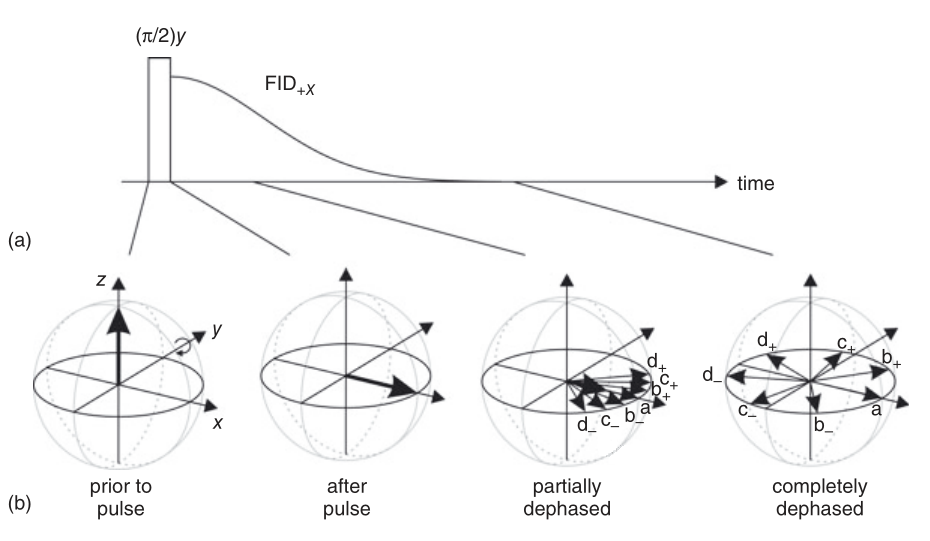
\includegraphics[width=0.9\textwidth]{images/2_stoll_fid}
		\caption{Schematic of pulse sequence and magnetic moment evolution of the spin packets in an FID experiment. (a) Pulse sequence, consisting of one $\pi/2$ pulse, and FID response. (b) In the rotating frame, after the $\pi/2$ pulse, the magnetic moment of individual spin packets precess at different frequencies. The total magnetic moment, indicated by the large arrow, decreases over time. Taken from \cite{stollPulseEPR2017}}
		\label{fig:2_stoll_fid}
	\end{figure}
	\section{Spin Hamiltonian}
	\label{sec:2_spin_H}
	Let's consider now the interaction of a spin with the magnetic field from a quantum mechanical point of view. The system is described by the so-called spin Hamiltonian, which in the frame of this work can be written as:
	\begin{equation}
		\mathcal{H}_0 =
		\mathcal{H}\tsub{Z} + \mathcal{H}\tsub{HFI} + \mathcal{H}\tsub{AB},
		\label{eq:2_spin_H}
	\end{equation}
	where $\mathcal{H}\tsub{Z}$ is the Zeeman interaction, $\mathcal{H}\tsub{HFI}$ is the hyperfine interaction term between the electron and nearby nuclei and $\mathcal{H}\tsub{AB}$ is the spin-spin interaction Hamiltonian, which accounts for interactions between multiple electrons. These terms will modify the form of the resonance peak. Other terms like the zero field splitting or the nuclear Zeeman interaction are neglected in the frame of this work. 
	
	\subsection{Zeeman Hamiltonian}
	As stated in section \ref{sec:2_basic_principles_EPR}, the g-value of an electron in a solid or in a molecular system differs from that of the free electron, $g\tsub{e}$. In this more complex case, the Zeeman Hamiltonian is given by:
	\begin{equation}
		\mathcal{H}\tsub{Z} =
		\mu\tsub{B} ( \mb{L} + g\tsub{e}\mb{S}) \cdot \mb{B}_0 + \lambda \mb{L} \cdot \mb{S}.
		\label{eq:2_Hz_spinorbit}
	\end{equation}
	To the free Zeeman Hamiltonian, two additional terms are present: the interaction between the angular momentum and the magnetic field and the spin-orbit coupling. Due to this latter term, the orbital eigenfunctions are admixed. In the majority of systems it is small compared to the other terms in the spin Hamiltonian, and thus can be considered as a perturbation. Making use of perturbation theory we can write the Zeeman Hamiltonian as:
	\begin{equation}
		\mathcal{H}\tsub{Z} =
		\mu\tsub{B} \mb{S} \cdot \mb{g} \cdot \mb{B}_0,
		\label{eq:2_Hz_tensor}
	\end{equation} 
	where the elements of the g-tensor $\mb{g}$ are:
	\begin{equation}
		g_{ij} = g_e\delta_{ij} + 2\lambda\sum_{n \neq 0}\frac{\bra{0}L_i\ket{n}\bra{n}L_j\ket{0}}{E_0 - E_n},
		\label{eq:2_gij_perturbtheory}
	\end{equation}
	where $\ket{0}$ and $\ket{n}$ are the wavefunctions of the ground and the n-th excited state with energies $E_0$ and $E_n$ respectively. % \textbf{copiato tutta la frase pari pari da Jannik}\\
	The tensor is symmetric, thus it can be diagonalized with a rotation. In the frame of reference of its principal axes, the g-tensor will have the form:
	\begin{equation}
		\mb{g}\tsub{diag} = 
		\left(
		\begin{array}{ccc}
			g_x	&&\\
			&g_y&\\
			&&g_z\\
		\end{array}
		\right).
		\label{eq:2_gdiag}
	\end{equation}
	With respect to this frame of reference, the magnetic field can be written as $\mb{B}_0 = B_0(\sin\theta\cos\phi, \sin\theta\sin\phi, \cos\theta)$, where $\theta$ is the polar and $\phi$ the azimuthal angle between the field and the frame. The measured g-value is thus given by:
	\begin{equation}
		g(\theta, \phi) = 
		\sqrt{(g_x\sin\theta\cos\phi)^2 + (g_y\sin\theta\sin\phi)^2 +  (g_z\cos\theta)^2}.
		\label{eq:2_g_measured}
	\end{equation}
	In case of rhombic symmetry, the three principal values $g_{x,y,z}$ are different and both angles $\theta$ and $\phi$ influence the measured g-value, as in Eq. \eqref{eq:2_g_measured}. If there is axial symmetry, the principal values can be written as $g_x = g_y = g_{\perp}$ and $g_z = g_\parallel$. These values can be observed respectively for $\mb{B}_0$ perpendicular and parallel to the symmetry axis. As a consequence, only the angle between the field and this axis needs to be specified, and the measured g-value is $g(\theta) = \sqrt{g_\parallel^2\cos^2\theta + g_\perp^2\sin^2\theta}$. If a cubic symmetry is present, all principal values are equal $g\tsub{x} = g\tsub{y} = g\tsub{z} = g$ and the measurement is not angular dependent.	
	
	\subsection{Hyperfine interaction}
	Analogous to electrons, nuclei have magnetic moments due to their spin $I$. The nuclear magnetic moment is given by:
	\begin{equation}
		\boldsymbol{\mu}\tsub{N} =
		\gamma\tsub{N}\hbar\mb{I} =
		g\tsub{N}\frac{e\hbar}{2m\tsub{p}}\mb{I} =
		g\tsub{N}\mu\tsub{N}\mb{I}.
		\label{eq:2_nuclear_mu}
	\end{equation}
	The definition is similar to the one given in Eq. \eqref{eq:2_electron_mu}, with the nuclear magneton $\mu\tsub{N} = e\hbar/2m\tsub{p}$ taking the place of Bohr magneton. Since $\mu\tsub{N}/\mu = m\tsub{e}/m\tsub{p} \simeq 10^{-3}$, the interaction of the nucleus with the external magnetic field, called nuclear Zeeman interaction, can be neglected when compared with the electron correspondent.\\
	The interaction between the electron and nuclear magnetic moment gives rise to the hyperfine interaction (HFI) term:
	\begin{equation}
		\mathcal{H}\tsub{HFI}/h = \mb{S} \cdot \mb{A} \cdot \mb{I},
	\end{equation}
	where $\mb{A}$ is the hyperfine-coupling tensor. Due to this interaction, the resonance spectrum will be split into $(2I+1)$ peaks, each one corresponding to a different nuclear spin state.\\
	The HFI can be separated into an isotropic term, called Fermi contact interaction, and the electron-nuclear dipolar interaction term. This is possible because the hyperfine-coupling tensor can be written as the sum of an isotropic and a traceless part:
	\begin{equation}
		\mb{A} = a\tsub{iso}\mb{I}_3 + \mb{T},
	\end{equation}
	where $\mb{I}_3$ is the identity matrix in three dimensions. The values of $a\tsub{iso}$ and of the dipolar tensor $\mb T$ can be obtained from classical electrodynamic theory using the point-dipole approximation for the two spins. For the isotropic hyperfine-coupling term, one obtains \cite{bennatiEPRInteractionsHyperfine2017}:
	\begin{equation}
		a\tsub{iso} =
		\frac{2}{3}\mu_0g\tsub e \mu\tsub B g\tsub N\mu\tsub N |\psi_0(r = 0)|^2 ,
		\label{eq:2_aiso}
	\end{equation}
	where $\mu_0$ is the vacuum permeability and $|\psi_0(r = 0)|^2$ is the probability of measuring the electron in the nucleus. $|\psi_0(r = 0)|^2 \neq 0$ only for s-type wavefunctions. The elements of the electron-nuclear coupling tensor are given by \cite{bennatiEPRInteractionsHyperfine2017}:
	\begin{equation}
		\label{eq:2_Tij}
		T_{ij} =
		\frac{\mu_0}{4\pi}g\tsub e \mu\tsub B g\tsub N\mu\tsub N
		\left <\psi_0\left |\frac{3r_ir_j - \delta_{ij}r^2}{r^5}\right |\psi_0 \right >
	\end{equation}
	where $\mb{r}$ is the distance vector from nucleus to electron.\\
	%	Since $\mb{T}$ is symmetric, it can be diagonalized
	%	\begin{equation}
	%		\mb{T}\tsub{diag} =
	%		\left(
	%		\begin{array}{ccc}
	%			T_x	&&\\
	%			&T_y&\\
	%			&&T_z\\
	%		\end{array}
	%		\right).
	%		\label{eq:2_Tdiag}
	%	\end{equation}
	%	\textbf{Qui aggiungo altro? T non è mai stata molto importante nei nostri esperimenti.}
	If a simple system of electron $S = 1/2$ and nuclear spin $I = 1/2$ is considered, the resulting spectra will present two peaks with a magnetic field difference equal to $a\tsub{iso}$. This is the case for phosphorus donors state in crystalline silicon: the resulting signal presents two peaks with a field splitting of $a\tsub{iso} = 4.2 \; \text{mT}$ \cite{feherElectronSpinResonance1959}.\\
	
	%	\subsection{Spin-spin interaction}
	%	The interaction between two spins gives rise to the spin-spin Hamiltonian
	%	\begin{equation}
	%		\label{eq:2_H_AB}
	%		\mathbf{H}\tsub{AB}/h = -J\mb S\tsub A \cdot \mb S\tsub B + \mb S\tsub A \cdot \mb D \cdot \mb S \tsub B,
	%	\end{equation}
	%	where the first term is the isotropic exchange interaction and the second term is the dipolar coupling. The exchange term takes into account the overlap of the orbitals of the spins. Depending on the sign of the exchange constant, the two spins will have ground state with total spin $S = 1$ ($J > 0$), which is referred to as ferromagnetic coupling, or ground state with total spin $S = 0$ ($J < 0$), in the antiferromagnetic state.\\
	%	The dipolar coupling term originates from dipole-dipole interactions. $\mathbf{D}$ is a traceless symmetric tensor, therefore can be diagonalized in a suitable base. In the limit of high-field conditions ($D \ll g\mu\tsub BB_0/h$) and using point-dipole approximation, the dipolar coupling term can be written as
	%	\begin{equation}
	%		\mb S\tsub A \cdot \mb D \cdot \mb S \tsub B =
	%		-D(3S_\text{A}^zS_\text{B}^z - \mathbf{S}\tsub A\cdot \mathbf{S}\tsub B) =
	%		-D(3\cos^2\theta -1),
	%	\end{equation}
	%	where $\theta$ is the angle between $\mb B_0$ and the distance between the two spins $\mb r\tsub{AB}$ and $D$ appears in the diagonal form of the dipolar tensor when written in the principla axis frame
	%	\begin{equation}
	%		\label{eq:2_Ddiag}
	%		\mb{D}\tsub{diag} =
	%		\left(
	%		\begin{array}{ccc}
	%			-D	&&\\
	%			&-D&\\
	%			&&2D\\
	%		\end{array}
	%		\right),
	%	\end{equation}
	%	where
	%	\begin{equation}
	%		D = \frac{\mu_0 g \tsub A g \tsub B \mu_\text B ^2}{4\pi h}\frac{1}{r_\text{AB}^3}.
	%	\end{equation}
	%	The dipolar coupling strength can derefore be used to determine the distance distribution of spin pairs.
	
	\section{Broadening of EPR lines}
	As previously discussed, the EPR spectrum will have an absorption line when the resonance criterion in Eq. \eqref{eq:2_nu_equal_nuL} is met. If every spin in the investigated sample had the same resonance condition, this would lead to a sharp peak for a certain field value. In this case, all the spins would belong to the same so-called spin packet. Both spin-lattice and spin-spin relaxation processes lead to a variety of spin packets with different resonance conditions, causing a broadening of the EPR line. In a usual experiment, both homogeneous and inhomogeneous line broadening take place.\\
	The minimum linewidth of a resonance peak is given by the Heisenberg uncertainty principle. As discussed in section \ref{sec:2_cwEPR}, the higher energy state has a finite lifetime. Transitions to the lower energy level due to interactions with the lattice happen with a time constant $T_1$. This process leads to a homogeneous broadening $\Gamma\tsub{hom} > 1/T_1$.\\
	Another source of homogeneous broadening comes from the distribution of Larmor frequencies due to local field inhomogeneity. The broadening that stems from this phenomenon is the dominant one in EPR experiments, therefore the resonant curve will be a Lorentzian with linewidth $\Gamma\tsub{hom} = 2/T_2$.\\
	Inhomogeneous line broadening can be caused by strain, distribution of Larmor frequencies due to local fluctuations of the magnetic field and unresolved hyperfine interactions. These effects lead to a distribution of spin packets with the resonance centered at different magnetic fields. As a result, the EPR resonance signal has a Gaussian lineshape of width $\Gamma\tsub{inh} > \Gamma\tsub{hom}$, as shown in Fig. \ref{fig:2_broadening}.
	\begin{figure}
		\centering
		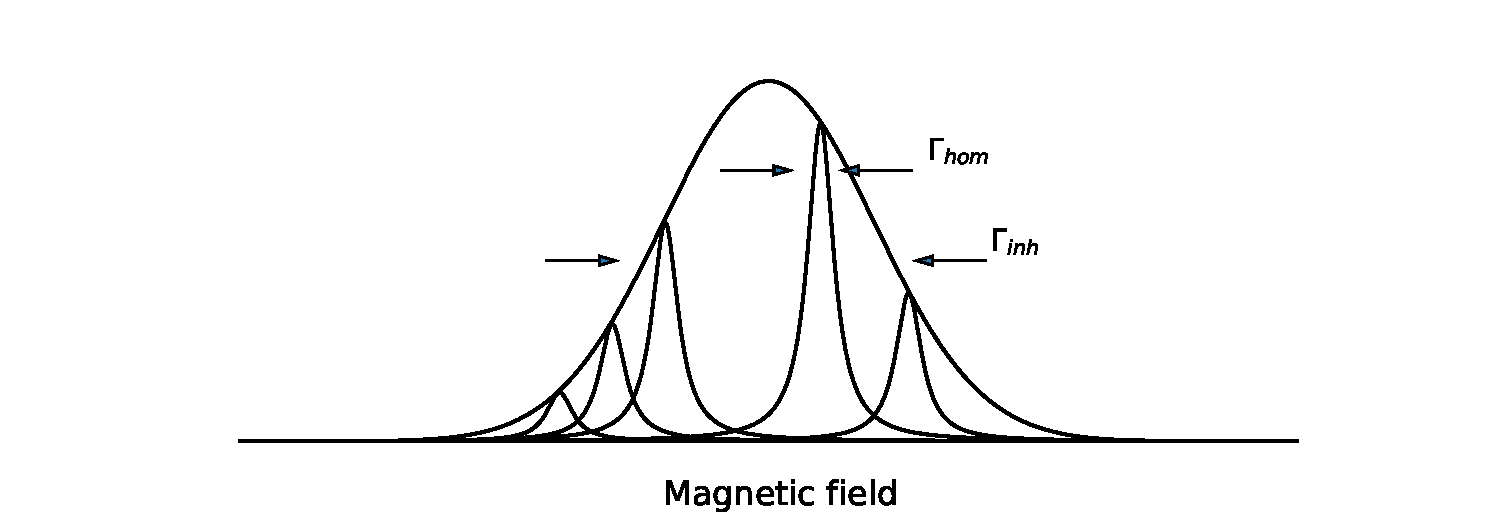
\includegraphics[width=\textwidth]{images/2_broadening}
		\caption{Lineshape of a resonance peak consisting of a superposition of different spin packets with homogeneous Lorentzian lineshape of width $\Gamma\tsub{hom}$. The resulting resonant peak has a Gaussian lineshape of width $\Gamma\tsub{inh}$. Adapted from \cite{schweigerPrinciplesPulseElectron2001}}
		\label{fig:2_broadening}
	\end{figure}
	
	\section{Basic principles of EDMR}
	The current-limiting defects in solar cells are paramagnetic, therefore they can be used as probes in EPR experiments \cite{lenahanWhatCanElectron1998}. Nevertheless, the characterization of these defects with EPR is in many cases not possible: EPR probes all the paramagnetic centers, thus not providing the selectivity to study only the defects that affect the current in the solar cell. Moreover, EPR does not provide the sensitivity required to detect defects in working devices, especially in state of the art solar cells where the number of defects in the active layer is below $10^{10} - 10^{13}$ spins \cite{schneggPulsedElectricallyDetected2012}.\\
	For these reasons, electrically detected magnetic resonance (EDMR) is the technique of choice in this work. EDMR is a spectroscopic method to study the electronic transitions of charge carriers through the measurement of current changes.
	
	\subsection{Spin-dependent electronic transitions}
	\label{sec:2_spin-dependent_electronic_processes}
	Using paramagnetic states as probes, EDMR gives information on the transport and recombination properties of the sample under investigation taking advantage of their spin dependent nature.\\
	Usually the spin is not a quantity of interest when studying the operation of a solar cell device because the spin orientation of an individual charge carrier is conserved only for short times at room temperature \cite{behrendsSpindependentTransportRecombination2009}. Nevertheless, the interaction between these particles and those occupying defect state levels is spin dependent.
	This is particularly important when considering materials with many defect levels in the bandgap, such as disordered semiconductors like amorphous silicon and interfaces between crystalline silicon and silicon dioxide (Si/SiO\tsub 2 interfaces).
	
	The first model attempting to explain the influence of EPR on the conductivity of a sample was proposed by Lepine in 1972 \cite{lepineSpinDependentRecombinationSilicon1972}. In Lepine's model, the resonant change of conductivity is explained by an increase of the capture cross section due to a change of thermal spin polarization of the free charge carriers and spin species occupying defect states. The dependence of the EDMR signal on the external microwave field and on the temperature predicted by this model does not explain several experimental results obtained in silicon \cite{streetSpindependentPhotoconductivityUndoped1982}\cite{brandtElectricallyDetectedMagnetic1998}.\\
	\begin{figure}
		\centering
		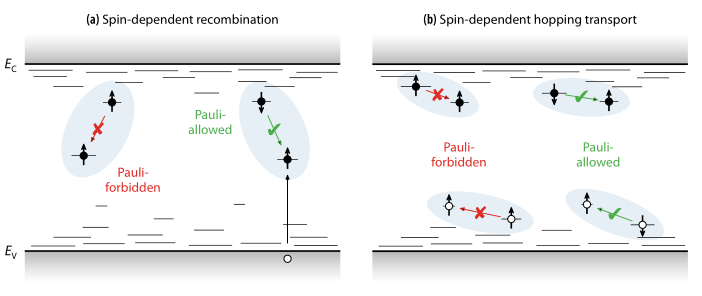
\includegraphics[width=\textwidth]{images/2_pauli_principle}
		\caption{Schematic of spin-dependent processes for charge carriers in amorphous silicon. Spin-dependent (a) recombination and (b) hopping is Pauli allowed only when the spins which form the spin pair are in an antiparallel configuration. Taken from ref. \cite{moserChargeTransportAmorphous2019}}
		\label{fig:2_pauli_principle}
	\end{figure}
	The weak dependence on these experimental parameters was explained in 1978 by Kaplan, Solomon and Mott (KSM) \cite{kaplanExplanationLargeSpindependent1978}. This model is based on the assumption that the interaction between free charge carriers and spin species occupying defect states happens through the formation of a weakly coupled spin pair. As shown in Fig. \ref{fig:2_pauli_principle}, when a semiconductor is placed into an external magnetic field transitions to energetically favorable configurations can be forbidden due to the Pauli exclusion principle: when the two spins are parallel, the transition is forbidden because two fermions % saying "electrons" here would exclude the case of two holes with the same spin configuration
	with the same spin configuration cannot occupy the same energetic state.\\
	After the formation of a spin pair, different processes can take place, each one with a different time constant \cite{stutzmannSpindependentProcessesAmorphous2000}:
	\begin{itemize}
		\item a spontaneous spin-flip can occur with a time constant equal to the spin-relaxation time $T_1$. After the spin-flip, the transition that was previously forbidden becomes allowed.
		\item if microwave radiation invests the sample, a resonant induced spin flip can take place with a time constant $\tau\tsub{SF} = 1/(\gamma B_1)$, where $\gamma$ is the gyromagnetic ratio and $B_1$ is the intensity of the microwave magnetic field.
		\item the spin pair can dissociate with a time constant $\tau\tsub{diss}$.
	\end{itemize}
	Additionally, when the spin pair is in an antiparallel configuration, a transition can happen with a time constant $\tau\tsub{trans}$. The transition can consist of two different processes, as shown in Fig. \ref{fig:2_pauli_principle}: recombination, where an electron and a hole annihilate through a midgap defect state, or hopping, where the spin species moves to a spatially adjacent energy state.\\
	In order to take advantage of spin resonance to effectively study electronic transitions, the condition to be met is:
	\begin{equation}
		\tau\tsub{trans} \ll \tau\tsub{SF} \ll T_1, \tau\tsub{diss}.
		\label{eq:3_tau_relations} 
	\end{equation}
	\begin{figure}
		\centering
		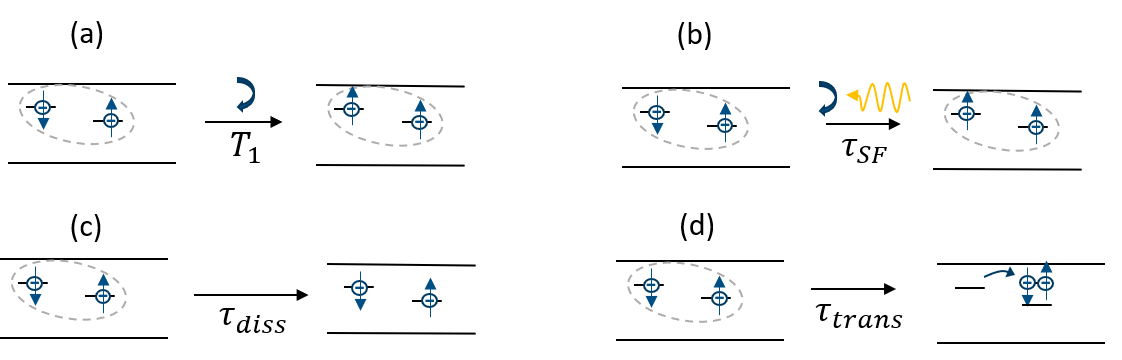
\includegraphics[width=0.9\textwidth]{images/2_stutzmann_transitions}
		\caption{Schematic of the possible processes following the formation of a spin pair. (a) Spontaneous spin-flip of one of the two spins. (b) Resonant spin-flip due to microwave radiation. (c) Dissociation of the spin pair. (d) Spin-dependent transition, either hopping (as shown here) or recombination. This last process can happen only when the spins of the spin pair are in an antiparallel configuration.}
		\label{fig:2_stutzmann_transitions}
	\end{figure}
	The spin-to-charge conversion that allows the measurement a changes in the current when resonant spin-flips occur will be discussed in section \ref{sec:2_spin-charge_conversion}.\\
	
	\subsection{Spin-pair Hamiltonian}
	\label{sec:2_spin-pair_H}
	According to the KSM model, at the basis of any spin-dependent electronic transition there is the formation of a coherent pair. It is of interest then to study the Hamiltonian describing a system of two spins with an external magnetic field $\mb{B_0}$
	\begin{equation}
		\mathcal{H}/h = 
		\frac{\mu\tsub B}{h} (\mb{S}\tsub A \cdot \mb{g}\textsubscript{A} + \mb{S} \tsub B \cdot \mb{g} \tsub B) \cdot \mb B_0 
		- J \mb{S} \tsub A \cdot \mb{S} \tsub B
		- D (3 S_\text A^z S^z_\text{B} - \mb{S}\tsub A \cdot \mb S\tsub B),
		\label{eq:2_spin-pair_H}
	\end{equation}
	where the first term is the sum of the Zeeman interaction of the two spins, while the other two terms are the exchange and dipolar coupling between the two spins. Neglecting for simplicity g-tensor anisotropy, we can write the spin-pair Hamiltonian in the product base $\ket{\psi} = \{ \ket{\uparrow\uparrow}, \ket{\uparrow\downarrow}, \ket{\downarrow\uparrow}, \ket{\downarrow\downarrow}\}$ as
	\begin{equation}
		\mathcal{H} = \frac{h}{2}
		\left(
		\begin{array}{cccc}
			2\nu_0 - \frac{J}{2} - D&&&\\
			&\Delta\nu + \frac{J}{2} + D&-J+D&\\
			&-J+D& -\Delta\nu + \frac{J}{2} + D&\\
			&&&-2\nu_0-\frac{J}{2}-D\\
		\end{array}
		\right),
		\label{eq:2_spin-pair_H_matrix}
	\end{equation}
	where $\nu_0 = (\nu\tsub{A} + \nu\tsub{B})/2$ is the mean Larmor frequency, $\nu \tsub{A,B} = g\tsub{A,B} \mu\tsub B B_0 / h$, and $\Delta\nu = \nu \tsub{A} - \nu\tsub{B}$ is the difference between the Larmor frequencies.\\
	The Hamiltonian can be diagonalized with an appropriate change of basis. The new eigenbasis is $\ket{\psi} = \{ \ket{T_+}, \ket{2}, \ket{3}, \ket{T_-}\}$, with:
	\begin{subequations}
		\label{eq:2_spin-pair_H_eigenstates}
		\begin{equation}		\ket{T_+} = \ket{\uparrow\uparrow},
		\end{equation}
		\begin{equation}
			\ket{2} = \cos \phi \ket{\uparrow\downarrow} -  \sin \phi \ket{\downarrow\uparrow},
		\end{equation}
		\begin{equation}			\ket{3} = \sin \phi \ket{\uparrow\downarrow} +  \cos \phi \ket{\downarrow\uparrow},
		\end{equation}
		\begin{equation}			\ket{T_-}  = \ket{\downarrow\downarrow},
		\end{equation}
	\end{subequations}
	where
	\begin{equation}
		\phi = \frac{1}{2}\arctan\frac{J-D}{\Delta\nu}
		\label{eq:2_spin-pair_H_mixing_angle}
	\end{equation}
	is called the mixing angle. In the new basis, the Hamiltonian has the form
	\begin{equation}
		\mathcal{H} = \frac{h}{2}
		\left(
		\begin{array}{cccc}
			2\nu_0 - \xi &&&\\
			&\nu_\Delta + \xi&&\\
			&& -\nu_\Delta + \xi&\\
			&&&-2\nu_\Delta-\xi\\
		\end{array}
		\right),
		\label{eq:2_spin-pair_H_matrix_diag}
	\end{equation}
	with
	\begin{equation}
		\nu_\Delta = \sqrt{(J-D)^2 + \Delta\nu^2}, \sss \xi = \frac{J}{2} + D.
		\label{eq:2_spin-pair_H_matrix_diag_2}
	\end{equation}
	For strongly coupled particles $|J - D| \gg \Delta\nu$, $\phi \rightarrow \pi / 4$ and the eigenvectors are given by the pure singlet and triplet state
	\begin{equation}
		\ket 2 = \ket S = \frac{1}{\sqrt{2}}(\ket{\uparrow\downarrow} - \ket{\downarrow\uparrow}), \sss 
		\ket 3 = \ket{T_0} = \frac{1}{\sqrt{2}}(\ket{\uparrow\downarrow} + \ket{\downarrow\uparrow}).
		\label{eq:2_spin-pair_H_pure_S_and_T0}
	\end{equation}
	In the limit of weak coupling strength $|J - D| \ll \Delta\nu$, $\phi \rightarrow 0$ and $\ket{2} = \ket{\uparrow\downarrow}$, $\ket 3 = \ket{\downarrow\uparrow}$. This is the case of spin-pair formation in KSM model.\\
	For intermediate cases, the eigenvectors will have a certain mixture of singlet and triplet content.\\
	
	\subsection{Spin-to-charge conversion}
	\label{sec:2_spin-charge_conversion}
	The electrical detection of recombination and hopping processes is based on the assumption that, when reaching magnetic resonance, the conductivity $\sigma$ of the sample changes. The total conductivity is given by the sum of the electron and hole conductivities:
	\begin{equation}
		\sigma = e(n\cdot \mu_e + p\cdot \mu_h),
		\label{eq:2_conductivity}
	\end{equation}
	where $e$ is the elemental charge, $n$ and $p$ are the density of electrons and holes and $\mu_e$ and $\mu_h$ are their respective mobilities. Magnetic resonance can generate a reduction of the density of charge carriers (recombination) or an increase in the mobility (hopping). A change in the conductivity implies a change in the current that flows through the device, consequently current detection can be used to investigate electronic transitions.\\
	As discussed in section \ref{sec:2_spin-dependent_electronic_processes}, according to KSM model the interaction between two spins starts with the formation of a weakly coupled spin pair. Afterwards, the presence of an EDMR signal is based on the Pauli exclusion principle. Therefore, the observable in an EDMR experiment is the spin-pair symmetry, in contrast with EPR where the observable is the spin polarization. In other words, the EDMR signal depends on the singlet and triplet content of the spin-pair ensemble. We can write the transition probability $p_i$ for a certain eigenstate $\ket{i}$ of the spin pair as \cite{boehmeInvestigationChargeCarrier2006}:
	\begin{equation}
		\label{eq:2_transition_probability}
		p_i =
		p_S|\braket{i|S}|^2 + p_T|\braket{i|T}|^2,
	\end{equation}
	where $p_S$ and $p_T$ are the transition probabilities for pure singlet and pure triplet states, respectively. Using Eqq. \eqref{eq:2_spin-pair_H_eigenstates} and Eqq. \eqref{eq:2_spin-pair_H_pure_S_and_T0}, one obtains the transition probabilities for the four eigenstates:
	\begin{equation}
		p_{T_+,T_-} = p_T, \sss p_{2,3} = \frac{p_S}{2}\left(1 \mp \frac{J-D}{\nu_\Delta}\right) + \frac{p_T}{2}\left(1 \pm \frac{J-D}{\nu_\Delta}\right). 
	\end{equation}
	Using a density matrix formalism, it is possible to calculate the evolution of the eigenstate populations under the spin Hamiltonian derived in section \ref{sec:2_spin_H}. Any change in the singlet or triplet content leads to an increase or decrease of the conductivity. In particular, recombination processes lead to a decrease of the density of charge carriers and hopping processes result in an increase of the mobility, with a consequent change of the conductivity (Eq. \eqref{eq:2_conductivity}) \cite{boehmeInvestigationChargeCarrier2006}\cite{boehmeInvestigationElectronicTransitions2004}. 
	
	\chapter{Materials and methods}
	In this chapter, the structure of the c-Si solar cell studied with Electrically Detected Magnetic Resonance and the experimental setup used in the course of this project are described.
	
	\section{c-Si minicell from NREL}
	The samples to be studied using EDMR have been produced by the National Renewable Energy Laboratory (NREL) in Golden, Colorado, USA. A schematic of the structure is shown in Fig. \ref{fig:3_minicells}. The absorber material is phosphorous-doped Czochralski (CZ) silicon. Silicon oxide SiO\tsub 2 is used to achieve passivation of the surface defects. A layer of polycrystalline silicon (poly-Si) surrounds the absorber layer to avoid edge shunts. On the top part of the solar cell, this poly-Si layer is highly n-doped, an anti-reflex coating is used to enhance the absorption of light and grid metal fingers are evaporated to extract charge carriers. On the back side, the poly-Si is highly p-doped and the metal back contact covers all the surface of the cell.
	\begin{figure}[b]
		\centering
		\begin{subfigure}{.65\textwidth}
			\centering
			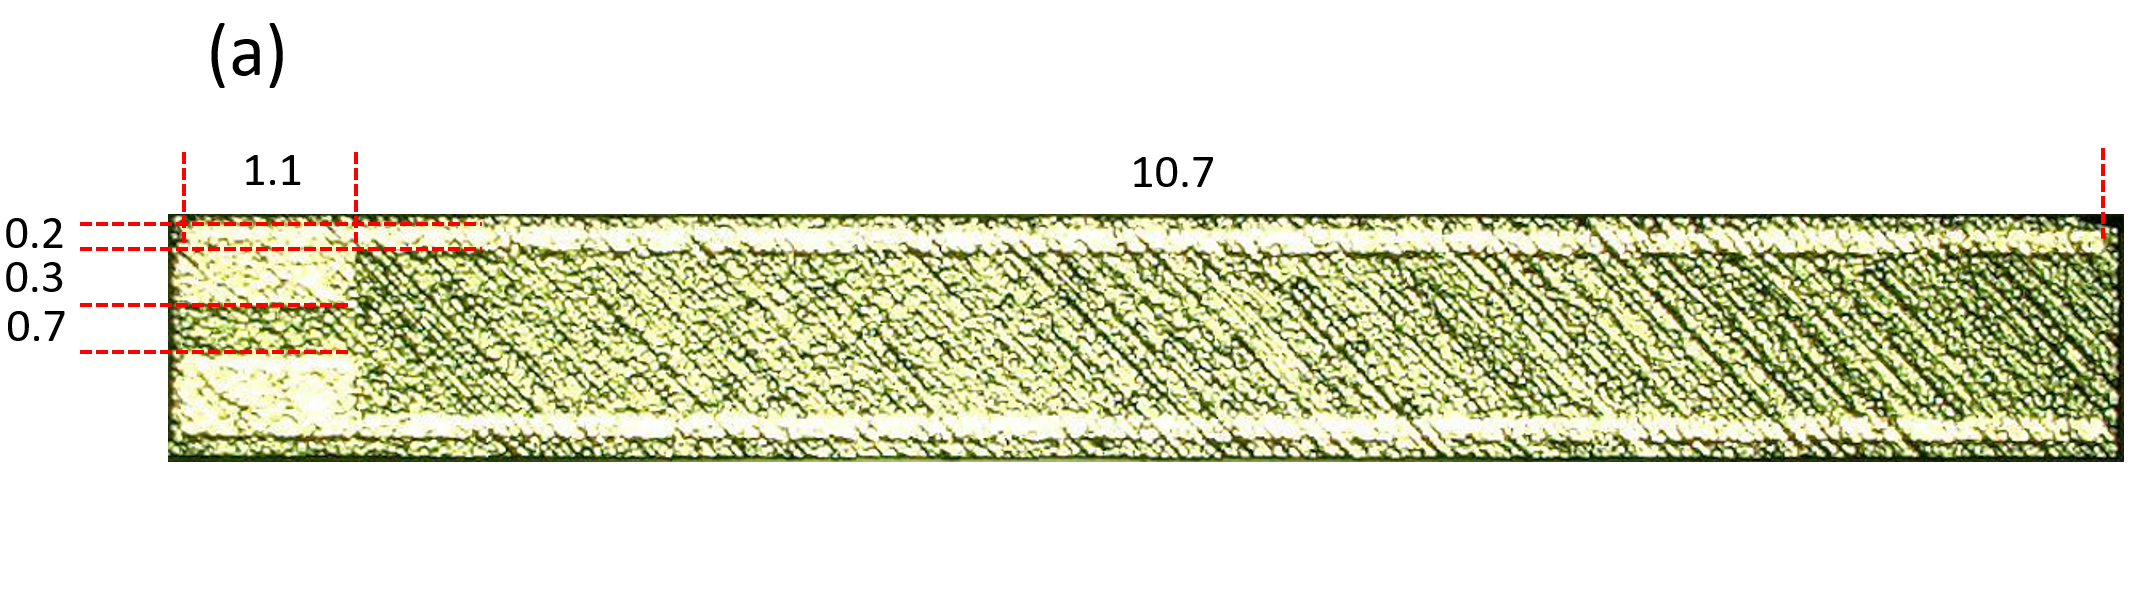
\includegraphics[width=\textwidth]{images/3_minicell_microscope.png}
		\end{subfigure}%
		\begin{subfigure}{.35\textwidth}
			\centering
			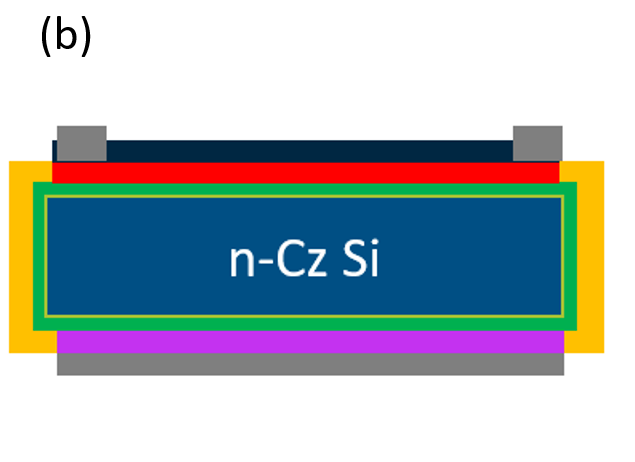
\includegraphics[width=.95\textwidth]{images/3_minicells.png}
		\end{subfigure}
		\caption{NREL solar cell structure. (a) Microscope image of the top view of the cell with dimensions in millimeters. (b) Schematic of the structure of the solar cell. The sample consists of n-doped Czochralski Si absorber (dark blue), SiO\tsub 2 passivation layer (green), poly-Si layer(intrinsic in yellow, n$^+$-doped in red, p$^+$-doped in purple), evaporated metal contacts (gray), anti-reflex coating (black). Figures from NREL, Golden, CO, USA.}
		\label{fig:3_minicells}
	\end{figure}
	
	\section{Experimental setup}
	\begin{figure}[t]
		\centering
		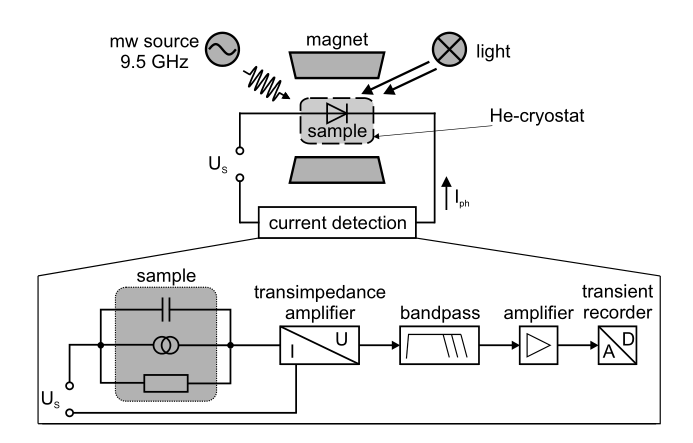
\includegraphics[width=0.9\textwidth]{images/3_behrends_exp_setup}
		\caption{Sketch of the experimental setup based on Bruker ELEXSYS E580 X-band EPR spectrometer. The sample is placed in a resonator inside a helium cryostat. A constant bias voltage $U_S$ can be applied, and light can be irradiated on the sample. The device (sketched with its circuital equivalent in the lower half of the picture) is connected through electrical contacts to the current detection scheme. \cite{behrendsSpindependentTransportRecombination2009}}
		\label{fig:3_behrends_exp_setup}
	\end{figure}
	The measurements presented in this work were carried out using an X-band EDMR setup based on a commercial Bruker ELEXSYS E580 X-band EPR spectrometer located in Helmholtz Zentrum Berlin (HZB) \cite{moserChargeTransportAmorphous2019}. The experimental setup is shown in Fig. \ref{fig:3_behrends_exp_setup}.\\
	The microwave radiation is generated by a continuous wave or pulsed MW bridge (Bruker E580-1010). An iron core electromagnet (Bruker ER 073) provides the required magnetic fields, up to a maximum of $1.45 \; \text T$. \\
	To enhance the microwave radiation at the sample, a dielectric-ring MW resonator (Bruker ER 4118X-MD-5) is used. To conduct experiments at low temperature, the resonator can be placed inside a liquid-helium cryostat (Bruker ER 4118CF). The temperature can be adjusted at constant helium flow using a temperature control unit (Oxford ITC503).\\
	An FT-NMR teslameter (Bruker ER 036TM) is used to measure the magnetic field outside of the cryostat. Standard EPR samples with known g-values (DPPH or N@C60) are used to calibrate the magnetic field \cite{pfluegerEndohedralAtomicNitrogen2012}: an offset is present due to the resonator and the cryostat walls, and due to fact that the sample is not placed at the same position as the teslameter.\\
	Light is shone onto the sample using an halogen cold light source (Schott KL 2500 LCD). The light enters the optical window of the cryostat and the resonator through a light guide. An external DC power supply (Thurlby Thandar TSX1820P) is used to increase the stability of the light source.\\
	To obtain high power microwave pulses a traveling-wave tube (TWT) amplifier (Applied Systems Engineering 1117X) is used. A multi-channel pulse-forming unit (MPFU) (Bruker PatternJet) is used to create the pulse sequences.\\
	The sample is inserted into an EPR quartz tube (outer diameter $4 \; \text{mm}$, inner diameter $3 \; \text{mm}$). Electrical wires are connected to the contact pads of the solar cell using silver paste and are then connected to the electrical detection system. \\
	The current detection is performed using a converter and amplifier (Elektronik-Manufaktur Mahlsdorf, EMM) specifically developed for EDMR experiments. The signal goes through a transimpendence amplifier (TIA) with a conversion factor of $10^4 \; \text{V/A}$, a band-pass filter where the high-pass cutoff removes the DC component of the signal while the low-pass cutoff determines the time resolution of the detection setup, and an additional amplifier. The signal is finally sent to the digitizer integrated into the spectrometer (Bruker SpecJet-II). Lock-in detection can be used in cwEDMR experiments to enhance the signal to noise ratio.\\
	
	
	%	\section{cwEDMR}
	%	In a continuous wave EDMR (cwEDMR) experiment, the sample is irradiated with microwave at constant frequency while the magnetic field is swept adiabatically.\\
	%	When the resonance condition of one of the two spins forming a spin pair is met, a change in the current will be measured. The signal to noise ratio is enhanced through the use of lock-in detection.\\
	%	A typical cwEDMR spectrum is shown in fig (\textbf{INSERT FIG}).
	%	
	%	\section{pEDMR}
	%	The advantage of pulsed EDMR (pEDMR) over cwEDMR experiment is in the possibility of studying the dynamics of the transition processes.\\
	%	The most basic and direct pulsed experiment is given by transient pEDMR. The sample, initially in equilibrium, is brought to a non-equilibrium state through a short and intense microwave pulse. The current change is measured as a function of time after. While the typical length of the pulse is of the order of tens to few hundreds of nanoseconds, the transient is recorded for more than a few hundread of microseconds, in order to study the dynamics until the sample is back to equilibrium.\\
	%	The transient is recorded for various values of the external magnetic field in order to obtain a 2D map. Fig (\textbf{Insert fig}) shows such a measurement.
	
	\chapter{Project plan}
	In this chapter, preliminary results of the EDMR measurements on the NREL c-Si solar cell will be briefly discussed. The data analysis of these measurements is still incomplete. Afterwards, the project plan regarding the EDMR measurements for the next months will be presented. Finally, the plan regarding the production of the heterojuction with intrinsic layer (HIT) solar cell will be discussed.
	
	\section{Preliminary results: cwEDMR on c-Si solar cell}
	Continuous wave EDMR (cwEDMR) spectra of the NREL c-Si solar cell under illumination are acquired for different values of the temperature. The measurements are shown in Fig. \ref{fig:4_cwEDMR_Tdependence}.
	%The cell was supplied with a reverse bias voltage $V\tsub{bias} = 1.10 \pm 0.01 \; \text{V}$.
	
	For $T \leq 16 \; \text K$, one can easily identify the signal coming from the phosphorus donor states, which consists of two peaks at a distance of $4.2 \; \text{mT}$ due to hyperfine interaction. Increasing the temperature, the thermal energy of the electrons 
	becomes comparable with the difference between the defect energy level and the conduction band edge ($40 \; \text{meV}$)\cite{feherElectronSpinResonance1959}. Thus an increasing number of phosphorus defects are ionized, leading to a decrease of the EDMR signal.
	
	A central peak is also distinguishable in all the spectra. The nature of this signal could be attributed to the presence of dangling bond defects at the interface between silicon and silicon dioxide (P\tsub b defect). Nevertheless, an initial data analysis suggests that the peak is the superposition of two different signals. The nature of the second one is still unclear: it could be due to dangling bonds at the grain boundaries of the highly doped poly-Si layers \cite{lipsDefectsRecombinationMicrocrystalline2003}; another possibility is that the signal stems from so-called E' defects in the bulk of the SiO\tsub 2 \cite{lenahanWhatCanElectron1998}\cite{ambalSpinRelaxationDynamicsCenters2015}. Further experiments are planned to clarify the nature of this current-limiting defect. In particular, experiments on symmetric structures, which are devices with the same doping of the poly-Si layer on both sides, are going to be helpful in isolating the different signals.\\
	\begin{figure}
		\centering
		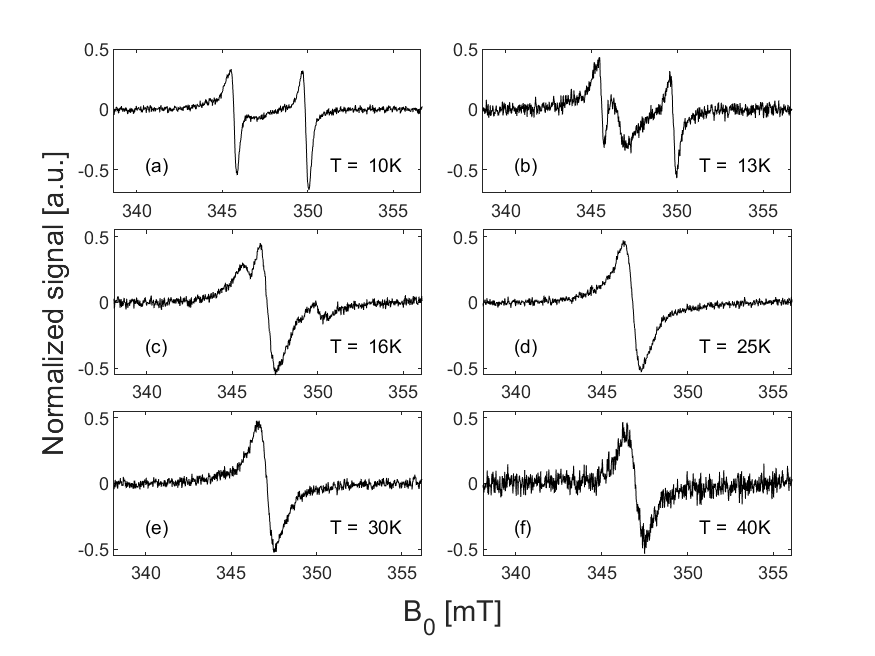
\includegraphics[width=\textwidth]{images/4_cwEDMR_Tdependence.png}
		\caption{Temperature dependence of the cwEDMR signals. The spectra (a), (b) and (c) show the typical $^{31}$P signal, with hyperfine splitting $\sim 4.2 \; \text{mT}$. The relative intensity of the central peak with respect to the $^{31}$P signal increases with increasing temperature. The nature of the central signal is still unclear.}
		\label{fig:4_cwEDMR_Tdependence}
	\end{figure}
	
	
	\section{Next steps: EDMR on c-Si solar cells and symmetric structures}
	\begin{figure}
		\centering
		\begin{subfigure}{.3\textwidth}
			\centering
			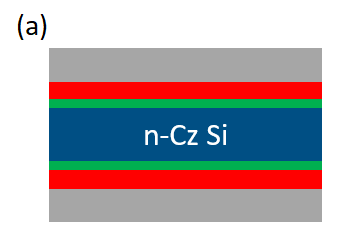
\includegraphics[width=\textwidth]{images/symmetric_structure_n.png}
		\end{subfigure}%
		\hspace{.1\textwidth}
		\begin{subfigure}{.32\textwidth}
			\centering
			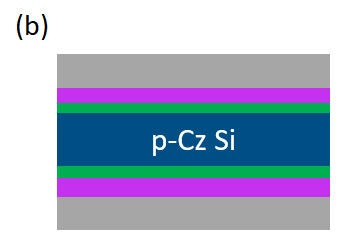
\includegraphics[width=.95\textwidth]{images/symmetric_structure_p.png}
		\end{subfigure}
		\caption{Sketches of symmetric structures. (a) n-doped Czochralski silicon absorber (dark blue), SiO\tsub 2 passivation layer (green), n-doped poly-Si (red), metal (gray). (b) p-doped Czochralski silicon absorber (dark blue), SiO\tsub 2 passivation layer (green), p-doped poly-Si (red), metal (gray).}
		\label{fig:4_symmetric_structures}
	\end{figure}
	As discussed in the previous section, a clear explanation of the results obtained so far is still missing. New samples are being produced by the NREL team. The new solar cells will be better suited for EDMR measurements: the active area will be reduced in size ($2 \; \text{mm}^2$); moreover, the back contact geometry will be modified to reduce the amount of metal inside the resonator. These modifications can ensure a more uniform magnetic field distribution all over the solar cell and reduce the field-dependent background signal generated by parasitic currents in the metal layer, hence enhancing the signal to noise ratio.
	
	It's still unclear at this stage from which layer is the signal coming from due to the complex structure of the solar cell. For this reason, the NREL team is producing devices with symmetric structures. In particular, two different structures are being realized: one, with n-doped poly-Si layer on both sides of the c-Si absorber; the other, with p-doped poly-Si on both sides. Sketches of the symmetric structures are shown in Fig. \ref{fig:4_symmetric_structures}. These symmetric structures can isolate signals that come from different parts of the device, helping to disentangle the various signals measured in the c-Si solar cell.
	
	Additionally, samples with boron doped crystalline silicon absorber are also being produced. Even though these solar cells have the largest commercial market share \cite{InternationalTechnologyRoadmap2021}, the processes of light induced degradation (LID), which leads to the formation of boron-oxygen complexes in the wafer of these devices, is still not completely understood. Previous research shows that these complexes reduce the efficiency of solar cells up to 5\% \cite{nieweltDegradationCrystallineSilicon2017}. The microscopic description that can be obtained through EDMR measurements can lead to a better physical understanding of the LID processes in the perspective of improving this technology.
	
	To summarize, the open questions that will be addressed in the next months are:
	\begin{itemize}
		\item identification of the processes that lead to the EDMR signals that were already observed in the phosporus doped c-Si solar cell.
		\item identification of the layers from which the EDMR signals come from.
		\item characterization of the boron-oxygen complexes in boron doped c-Si solar cells.
	\end{itemize}
	The project plan for the next months follows:
	\begin{itemize}
		\item January 2022: temperature dependence of the EDMR signal on the new solar cells with n-doped absorber. The goal of these experiments is to reproduce with a better signal to noise ratio the signals that were observed in the first sample. Moreover, temperature dependent EDMR measurements will be carried out on the p-doped c-Si solar cells.
		\item February 2022: temperature dependence of the EDMR signal on the symmetric structures to disentangle and understand the nature of the different signals that were observed in the n-doped c-Si solar cell.
		\item March 2022: angular dependence of the EDMR signal on all samples, with the goal of identify the signals that are dependent on the angle between the surface of the cell and the external magnetic field. The initial interpretation that the signal comes from the P\tsub b defect at the Si/SiO\tsub 2 interface will be either confirmed or disproved.
		\item March - May 2022: data analysis and writing of the master thesis.		
	\end{itemize}
	
	\section{Production of HIT solar cells}
	The second part of my master thesis is dedicated to the production of heterojunction with intrinsic layer (HIT) solar cells. This is a more technical side project, in which I  take care sample production in collaboration with the PVcomB department of the Helmholtz Zentrum Berlin (HZB). In particular, I am involved in the realization of the masks for the deposition of the various layers of the solar cell; moreover, I will take care the laser cutting process with the aim of finding the right parameters for the UV Keyence laser that lead to the formation of the lowest possible amount of defect states.\\
	Once the solar cells are produced, measurements will be carried out on the samples to ensure that they are working and that they show an EDMR signal, which is expected to stem from the a-Si layers.\\
	The project plan for the next months follows:
	\begin{itemize}
		\item December 2021 - February 2022: creation of masks for the deposition of the different layers; study of the dependence of the laser cutting process on the various laser parameters. 
		\item March 2022: EDMR measurements on the produced samples.
		\item March - May 2022: data analysis and writing of the master thesis.		
	\end{itemize}
	
	\printbibliography
\end{document}



